\documentclass[]{article}

% Imported Packages
%------------------------------------------------------------------------------
\usepackage{amssymb}
\usepackage{amstext}
\usepackage{amsthm}
\usepackage{amsmath}
\usepackage{enumerate}
\usepackage{fancyhdr}
\usepackage[margin=1in]{geometry}
\usepackage{graphicx}
\usepackage{extarrows}
\usepackage{setspace}
%------------------------------------------------------------------------------

% Header and Footer
%------------------------------------------------------------------------------
\pagestyle{plain}  
\renewcommand\headrulewidth{0.4pt}                                      
\renewcommand\footrulewidth{0.4pt}                                    
%------------------------------------------------------------------------------

% Title Details
%------------------------------------------------------------------------------
\title{Deliverable \#3 Template}
\author{SE 3A04: Software Design II -- Large System Design}
\date{}                               
%------------------------------------------------------------------------------

% Document
%------------------------------------------------------------------------------
\begin{document}

\maketitle	

\section{Introduction}
\label{sec:introduction}
% Begin Section

This section should provide an brief overview of the entire document.

\subsection{Purpose}
\label{sub:purpose}
% Begin SubSection
\begin{enumerate}[a)]
	\item Delineate the purpose of the document
	\item Specify the intended audience for the document
\end{enumerate}
% End SubSection

\subsection{System Description}
\label{sub:system_description}
% Begin SubSection
\begin{enumerate}[a)]
	\item Give a brief description of the system. This could be a paragraph or two to give some context to this document.
\end{enumerate}
% End SubSection

\subsection{Overview}
\label{sub:overview}
% Begin SubSection
\begin{enumerate}[a)]
	\item Describe what the rest of the document contains 
	\item Explain how the document is organised
\end{enumerate}

% End SubSection

% End Section

\section{State Charts for Controller Classes}
\label{sec:state_charts_for_controller_classes}
% Begin Section
This section should provide a state chart for each controller class for your application.
% End Section

\section{Sequence Diagrams}
\label{sec:sequence_diagrams}
% Begin Section
This section should provide a sequence diagram for each use case of your application.
% End Section

\section{Detailed Class Diagram}
\label{sec:detailed_class_diagram}
% Begin Section
This section should provide a detailed class diagram for your application.
% End Section

\appendix
\section{Division of Labour}
\label{sec:division_of_labour}
% Begin Section
\subsection{Ahsan Muzammil}
\begin{itemize}
  \item Section 3.1: Wrote about the different architecture designs we considered but eliminated.
  \item Section 3.2: Wrote about each subsystem and how they interact with each other.
  \item \textbf{Class Responsibility Cards:} Contributed to four CRC cards:
        \begin{itemize}
          \item View Car Depreciation Curve
          \item Request Car Recommendation
          \item Extended AI Service
          \item View Car Recommendation
        \end{itemize}
  \item Suggested changes to the Analysis Class Diagram.
        \begin{center}
          
\includegraphics[scale=0.1]{ahsan.jpeg}
        \end{center}
\end{itemize}

\subsection{Rebecca Di Filippo}
\begin{itemize}
  \item Wrote Section 1.1: Purpose of Document
  \item Wrote Section 1.2:  System Description
  \item Wrote Section 1.3: Overview of Document
  \item Contributed 4 Class Responsibility Cards
        \begin{itemize}
          \item Registration
          \item Login
          \item Account Information
          \item View Account
        \end{itemize}
        \begin{center}
          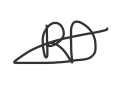
\includegraphics[scale=1.2]{rebecca.png}
        \end{center}
\end{itemize}

\subsection{Ethan Walsh}
\begin{itemize}
  \item Section 3: Derived initial system diagram.
  \item Section 3: Proposed edits to updated system diagram.
  \item Section 3: Wrote initial description of system architecture
  \item Section 3: Wrote description of used architecture styles and rationale
  \item Section 3: Wrote part of section 3.2, Subsystems
  \item Contributed 4 Class Responsibility Cards
        \begin{itemize}
          \item Experts Process Management
          \item Edit Account
          \item Request Information
          \item Account Error
        \end{itemize}
        \begin{center}
          
\includegraphics[scale=0.7]{ethan.png}
        \end{center}
\end{itemize}

\subsection{Jake Finlay}
\begin{itemize}
  \item Came up with some classes for the initial Analysis Class Diagram
  \item Contributed 9 Class Responsibility Cards
        \begin{itemize}
          \item Experts Service
          \item Point System Algorithm Expert
          \item External API Service Expert
          \item Redbook API
          \item AI Expert
          \item AI API
          \item Deal Report Management
          \item View Car Deal Report
          \item Save Car Deal Report
        \end{itemize}
  \item Helped with conversion to Latex
        \begin{center}
          
\includegraphics[scale=0.6]{jake.png}
        \end{center}
\end{itemize}

\subsection{Omer Karo}
\begin{itemize}
  \item created initial analysis class diagram for the car recommendation service subsystem
  \item created initial analysis class diagram for the deal report management subsystem
  \item created initial analysis class diagram for the experts process management
  \item Contributed 4 Class Responsibility Cards
        \begin{itemize}
          \item Request Intake
          \item Response Handler
          \item Car Recommendation service
          \item Request Car Depreciation Curve
        \end{itemize}
  \item Helped with conversion to Latex
        \begin{center}
          
\includegraphics[scale=0.2]{omer.jpg}
        \end{center}
\end{itemize}

\subsection{Abdallah Alqashqish}
\begin{itemize}
  \item Section 2: Collaborated on the Analysis Class Diagram (created and determined initial functionality of)
        \begin{itemize}
          \item Account Management Controller.
          \item Experts service.
          \item Refactored experts that depend on API to use a controller and boundary.
        \end{itemize}
  \item Section 3.1: Refined system architecture diagram to match the final agreed upon architecture.
  \item Contributed 4 Class Responsibility Cards
        \begin{itemize}
          \item Car Recommendation Information (Entity).
          \item Account Management (Controller).
          \item Logout (Boundary).
          \item Account Success (Boundary).
        \end{itemize}
        \begin{center}
          
\includegraphics[scale=0.1]{abdallah.jpg}
        \end{center}
\end{itemize}
% End Section

\newpage
\section*{IMPORTANT NOTES}
\begin{itemize}
	\item You do \underline{NOT} need to provide a text explanation of each diagram; the diagram should speak for itself
	\item Please document any non-standard notations that you may have used
	\begin{itemize}
		\item \emph{Rule of Thumb}: if you feel there is any doubt surrounding the meaning of your notations, document them
	\end{itemize}
	\item Some diagrams may be difficult to fit into one page
	\begin{itemize}
		\item It is OK if the text is small but please ensure that it is readable when printed
		\item If you need to break a diagram onto multiple pages, please adopt a system of doing so and throughly explain how it can be reconnected from one page to the next; if you are unsure about this, please ask me
	\end{itemize}
	\item Please submit the latest version of Deliverable 1 and Deliverable 2 with Deliverable 3
	\begin{itemize}
		\item They do not have to be a freshly printed versions; the latest marked versions are OK
	\end{itemize}
	\item If you do \underline{NOT} have a Division of Labour sheet, your deliverable will \underline{NOT} be marked
\end{itemize}


\end{document}
%------------------------------------------------------------------------------